\documentclass[[12pt,twoside]{book}
\usepackage{_my_document_style}
\begin{document}
%
\def\mySweepLEWingIDEG{32.200000}
\def\mySweepLEWingIIDEG{32.200000}
\def\mySweepLEWingIRAD{0.561996}
\def\mySweepLEWingIIRAD{0.561996}
\def\mySweepTEWingIDEG{3.800000}
\def\mySweepTEWingIIDEG{21.300000}
\def\mySweepTEWingIRAD{0.066323}
\def\mySweepTEWingIIRAD{0.371755}
\def\mySpanWingMT{58.670000}
\def\mySpanWingIMT{19.360000}
\def\mySpanWingIIMT{39.310000}
\def\myChordRootWingMT{11.870000}
\def\myChordRootWingIMT{11.870000}
\def\myChordRootWingIIMT{6.420000}
\def\myChordTipWingMT{1.690000}
\def\myChordTipWingIMT{6.420000}
\def\myChordTipWingIIMT{1.690000}
\def\mySweepLEWingIIDEG{32.200000}
\def\myCoeffAChordWingI{-0.563017}
\def\myCoeffBChordWingIMT{11.870000}
\def\myCoeffAChordWingII{-0.240651}
\def\myCoeffBChordWingIIMT{6.420000}
\def\myAlphaZeroLiftRootWingIDEG{-2.500000}
\def\myAlphaZeroLiftTipWingIDEG{-2.500000}
\def\myAlphaZeroLiftRootWingIRAD{-0.043633}
\def\myAlphaZeroLiftTipWingIRAD{-0.043633}
\def\myAlphaZeroLiftRootWingIIDEG{-2.500000}
\def\myAlphaZeroLiftTipWingIIDEG{-1.000000}
\def\myAlphaZeroLiftRootWingIIRAD{-0.043633}
\def\myAlphaZeroLiftTipWingIIRAD{-0.017453}
\def\myTaperRatioWingI{0.540859}
\def\myTaperRatioWingII{0.263240}
\def\myTwistWingIDEG{0.000000}
\def\myTwistWingIRAD{0.000000}
\def\myTwistWingIIDEG{-3.000000}
\def\myTwistWingIIRAD{-0.052360}
\def\myAreaWingIMTsquared{177.047200}
\def\myAreaWingIIMTsquared{159.402050}
\def\myCLAlphaRootWingIRAD{6.150000}
\def\myCLAlphaRootWingIDEG{0.107338}
\def\myCLAlphaRootWingIIRAD{6.050000}
\def\myCLAlphaRootWingIIDEG{0.105592}
\def\myCLAlphaTipWingIRAD{6.050000}
\def\myCLAlphaTipWingIDEG{0.105592}
\def\myCLAlphaTipWingIIRAD{6.010000}
\def\myCLAlphaTipWingIIDEG{0.104894}
\def\myXsiacRootWingI{0.250000}
\def\myXsiacTipWingI{0.250000}
\def\myXsiacRootWingII{0.250000}
\def\myXsiacTipWingII{0.250000}
\def\myCmZeroRootWingI{-0.080000}
\def\myCmZeroTipWingI{-0.080000}
\def\myCmZeroRootWingII{-0.080000}
\def\myCmZeroTipWingII{-0.040000}
\def\myMach{0.650000}
\def\myMACWingIMT{9.415662}
\def\myMACWingIIMT{4.514780}
\def\myMACWingCrankedMT{7.093735}
\def\myAreaWingCrankedMTsquared{336.449250}
\def\myAspectRatioWingCranked{10.230871}
\def\myXMACLEToApexWingIMT{2.745175}
\def\myAspectRatioWingI{2.117004}
\def\myAspectRatioWingII{9.694205}
\def\myYMACWingIMT{4.359264}
\def\myXMACLEToApexWingIIMT{4.985559}
\def\myYMACWingIIMT{17.596934}
\def\myYYMACWingCrankedMT{8.483347}
\def\myXXMACLEToApexWingCrankedMT{5.342249}
\def\myKOneACDatcomWingI{1.259000}
\def\myKTwoACDatcomWingI{0.242000}
\def\myXACOverChordRootDatcomWingI{0.411000}
\def\myXACOverChordRootDatcomWingII{0.958000}
\def\myChordRootWingIIPrimeMT{7.584752}
\def\myTaperRatioWingIIPrime{0.222815}
\def\mySpanWingIIPrimeMT{48.990000}
\def\myAreaWingIIPrimeMTsquared{227.185050}
\def\myAspectRatioWingIIPrime{10.564164}
\def\myCLAlphaAtMACWingRAD{7.289727}
\def\myCLAlphaPolhamusWingIRAD{2.835354}
\def\myCLAlphaPolhamusWingIDEG{0.049486}
\def\myCLAlphaPolhamusWingIIRAD{5.923041}
\def\myCLAlphaPolhamusWingIIDEG{0.103377}
\def\myXsiACWing{0.601251}
\def\myACWingToApexWingMT{9.607364}
\def\myXsiACWingI{0.212771}

%
\begin{figure}[t]%[H]%[!htbp]
  %\centering
  %\checkoddpage
  %\centering
    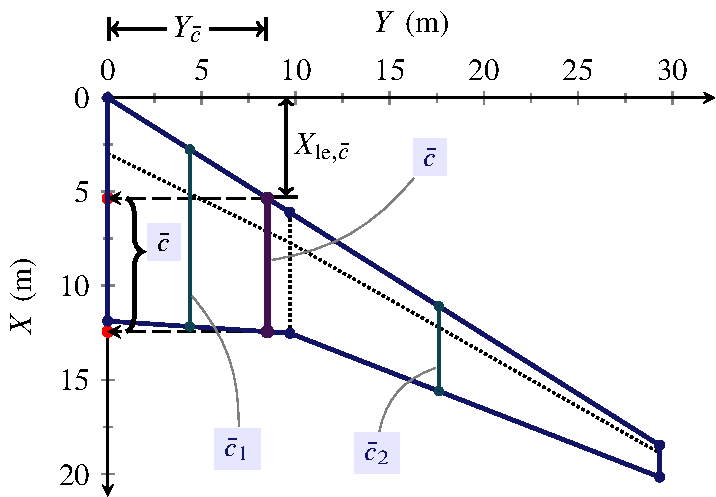
\includegraphics[width=0.78\textwidth]{Chapter_2/aerodynamic_center_of_a_cranked_wing/wing_ac_cranked_1_drawing_mac.pdf}
  \caption{\finalhyphendemerits=1000
         Aerodynamic mean chord of the wing proposed in the example~\ref{example:Wing:Aerodynamic:Center:Cranked}.
  }
  \label{fig:Wing:Aerodynamic:Center:Cranked:MAC}%
\end{figure}
%
\begin{myExampleX}{Aerodynamic center of a cranked wing}{\ding{46}\ \myIconGraph\ }% \ \Keyboard\ %
\label{example:Wing:Aerodynamic:Center:Cranked}
%
\noindent
In this example the position of the aerodynamic center will be calculated
of a wing similar to that of a Boeing~787.
The wing considered is of type \emph{cranked}, as can be seen from the planform shown in
figure~\ref{fig:Wing:Aerodynamic:Center:Cranked:Panels},and has the following characteristics:

\smallskip
\noindent
\adjustbox{center=\textwidth}{%
 \underline{\emph{Panel 1} (inner panel)}
}

\smallskip
\noindent
\adjustbox{left=\textwidth}{%
  \adjustbox{right=0.39\textwidth}{%
    \emph{chords}:
  }\rule{0.5em}{0pt}% --> SPACER
  \adjustbox{left=0.59\textwidth}{%
    $c_{\mathrm{r},1}=\SI[round-precision=2]{\myChordRootWingIMT}{\metre}$,
    $c_{\mathrm{t},1}=\SI[round-precision=2]{\myChordTipWingIMT}{\metre}$,
    $\lambda_1 = \SI[round-precision=2]{\myTaperRatioWingI}{}$,
  }%
}

\smallskip
\noindent
\adjustbox{left=\textwidth}{%
  \adjustbox{right=0.39\textwidth}{%
    \emph{wingspan and wing surface}:
  }\rule{0.5em}{0pt}% --> SPACER
  \adjustbox{left=0.59\textwidth}{%
    $b_1=\SI[round-precision=2]{\mySpanWingIMT}{\metre}$,
    $S_1=\SI[round-precision=2]{\myAreaWingIMTsquared}{\meter^2}$,
    $\AR_1 = \SI[round-precision=2]{\myAspectRatioWingI}{}$,
  }%
}

\smallskip
\noindent
\adjustbox{left=\textwidth}{%
  \adjustbox{right=0.39\textwidth}{%
    \emph{sweep angles}:
  }\rule{0.5em}{0pt}% --> SPACER
  \adjustbox{left=0.59\textwidth,minipage=[t]{0.59\textwidth}}{%
    $\Lambda_\mathrm{le,1}=\SI[round-precision=4]{\mySweepLEWingIRAD}{\radian}=\SI[round-precision=1]{\mySweepLEWingIDEG}{\deg}$,
    \\
    $\Lambda_\mathrm{te,1}=\SI[round-precision=4]{\mySweepTEWingIRAD}{\radian}=\SI[round-precision=1]{\mySweepTEWingIDEG}{\deg}$,
  }%
}

\smallskip
\noindent
\adjustbox{left=\textwidth}{%
  \adjustbox{right=0.39\textwidth}{%
    \emph{gradient $C_{\ell_\mathlarger{\alpha}}$ of profile}:
  }\rule{0.5em}{0pt}% --> SPACER
  \adjustbox{left=0.59\textwidth,minipage=[t]{0.59\textwidth}}{%
    $C_{\ell_\mathlarger{\alpha},\mathrm{r},1}=\SI[round-precision=2]{\myCLAlphaRootWingIRAD}{\radian^{-1}}=\SI[round-precision=4]{\myCLAlphaRootWingIDEG}{\deg^{-1}}$,
    \\
    $C_{\ell_\mathlarger{\alpha},\mathrm{t},1}=\SI[round-precision=2]{\myCLAlphaTipWingIRAD}{\radian^{-1}}=\SI[round-precision=4]{\myCLAlphaTipWingIDEG}{\deg^{-1}}$,
  }%
}

\smallskip
\noindent
\adjustbox{left=\textwidth}{%
  \adjustbox{right=0.39\textwidth}{%
    \emph{twist}:
  }\rule{0.5em}{0pt}% --> SPACER
  \adjustbox{left=0.59\textwidth,minipage=[t]{0.59\textwidth}}{%
    $\alpha_{0\ell,\mathrm{r},1}=\SI[round-precision=3]{\myAlphaZeroLiftRootWingIRAD}{\radian}
      =\SI[round-precision=1]{\myAlphaZeroLiftRootWingIDEG}{\deg}$,\\
    $\alpha_{0\ell,\mathrm{t},1}=\SI[round-precision=3]{\myAlphaZeroLiftTipWingIRAD}{\radian}
      =\SI[round-precision=1]{\myAlphaZeroLiftTipWingIDEG}{\deg}$,\\
    $\epsilon_{\mathrm{g,t},1}=\SI[round-precision=0]{\myTwistWingIRAD}{\radian}
      =\SI[round-precision=0]{\myTwistWingIDEG}{\deg}$,
  }%
}

\smallskip
\noindent
\adjustbox{left=\textwidth}{%
  \adjustbox{right=0.39\textwidth}{%
    \emph{aerodynamic profile centers}:
  }\rule{0.5em}{0pt}% --> SPACER
  \adjustbox{left=0.59\textwidth}{%
    $\bar{x}_{\mathrm{ac,2D,1},\mathrm{r}}=\SI[round-precision=2]{\myXsiacRootWingI}{}$,
    $\bar{x}_{\mathrm{ac,2D,1},\mathrm{t}}=\SI[round-precision=2]{\myXsiacTipWingI}{}$,
  }%
}

\smallskip
\noindent
\adjustbox{left=\textwidth}{%
  \adjustbox{right=0.39\textwidth}{%
    \emph{coefficients $C_{\mathcal{m}_\mathlarger{\mathrm{ac}}}$ of profile}:
  }\rule{0.5em}{0pt}% --> SPACER
  \adjustbox{left=0.59\textwidth}{%
    $C_{\mathcal{m}_\mathlarger{\mathrm{ac}},\mathrm{r},1}=\SI[round-precision=3]{\myCmZeroRootWingI}{}$,
    $C_{\mathcal{m}_\mathlarger{\mathrm{ac}},\mathrm{t},1}=\SI[round-precision=3]{\myCmZeroTipWingI}{}$,
  }%
}

\medskip
\noindent
\adjustbox{center=\textwidth}{%
 \underline{\emph{Pannello 2} (outer pannel)}
}

\smallskip
\noindent
\adjustbox{left=\textwidth}{%
  \adjustbox{right=0.39\textwidth}{%
    \emph{chords}:
  }\rule{0.5em}{0pt}% --> SPACER
  \adjustbox{left=0.59\textwidth}{%
    $c_{\mathrm{r},2}=\SI[round-precision=2]{\myChordRootWingIIMT}{\metre}$,
    $c_{\mathrm{t},2}=\SI[round-precision=2]{\myChordTipWingIIMT}{\metre}$,
    $\lambda_2 = \SI[round-precision=2]{\myTaperRatioWingII}{}$,
  }%
}

\smallskip
\noindent
\adjustbox{left=\textwidth}{%
  \adjustbox{right=0.39\textwidth}{%
    \emph{wingspan and wing surface}:
  }\rule{0.5em}{0pt}% --> SPACER
  \adjustbox{left=0.59\textwidth}{%
    $b_2=\SI[round-precision=2]{\mySpanWingIIMT}{\metre}$,
    $S_2=\SI[round-precision=2]{\myAreaWingIIMTsquared}{\meter^2}$,
    $\AR_2 = \SI[round-precision=2]{\myAspectRatioWingII}{}$,
  }%
}

\smallskip
\noindent
\adjustbox{left=\textwidth}{%
  \adjustbox{right=0.39\textwidth}{%
    \emph{sweep angles}:
  }\rule{0.5em}{0pt}% --> SPACER
  \adjustbox{left=0.59\textwidth,minipage=[t]{0.59\textwidth}}{%
    $\Lambda_\mathrm{le,2}=\SI[round-precision=4]{\mySweepLEWingIIRAD}{\radian}=\SI[round-precision=1]{\mySweepLEWingIIDEG}{\deg}$,
    \\
    $\Lambda_\mathrm{te,2}=\SI[round-precision=4]{\mySweepTEWingIIRAD}{\radian}=\SI[round-precision=1]{\mySweepTEWingIIDEG}{\deg}$,
  }%
}

\smallskip
\noindent
\adjustbox{left=\textwidth}{%
  \adjustbox{right=0.39\textwidth}{%
    \emph{gradients $C_{\ell_\mathlarger{\alpha}}$ of profile}:
  }\rule{0.5em}{0pt}% --> SPACER
  \adjustbox{left=0.59\textwidth,minipage=[t]{0.59\textwidth}}{%
    $C_{\ell_\mathlarger{\alpha},\mathrm{r},2}=\SI[round-precision=2]{\myCLAlphaRootWingIIRAD}{\radian^{-1}}=\SI[round-precision=4]{\myCLAlphaRootWingIIDEG}{\deg^{-1}}$,
    \\
    $C_{\ell_\mathlarger{\alpha},\mathrm{t},2}=\SI[round-precision=2]{\myCLAlphaTipWingIIRAD}{\radian^{-1}}=\SI[round-precision=4]{\myCLAlphaTipWingIIDEG}{\deg^{-1}}$,
  }%
}

\smallskip
\noindent
\adjustbox{left=\textwidth}{%
  \adjustbox{right=0.39\textwidth}{%
    \emph{twist}:
  }\rule{0.5em}{0pt}% --> SPACER
  \adjustbox{left=0.59\textwidth,minipage=[t]{0.59\textwidth}}{%
    $\alpha_{0\ell,\mathrm{r},2}=\SI[round-precision=3]{\myAlphaZeroLiftRootWingIIRAD}{\radian}
      =\SI[round-precision=1]{\myAlphaZeroLiftRootWingIIDEG}{\deg}$,\\
    $\alpha_{0\ell,\mathrm{t},2}=\SI[round-precision=3]{\myAlphaZeroLiftTipWingIIRAD}{\radian}
      =\SI[round-precision=1]{\myAlphaZeroLiftTipWingIIDEG}{\deg}$,\\
    $\epsilon_{\mathrm{g,t},2}=\SI[round-precision=3]{\myTwistWingIIRAD}{\radian}
      =\SI[round-precision=1]{\myTwistWingIIDEG}{\deg}$,
  }%
}

\smallskip
\noindent
\adjustbox{left=\textwidth}{%
  \adjustbox{right=0.39\textwidth}{%
    \emph{aerodynamic profile centers}:
  }\rule{0.5em}{0pt}% --> SPACER
  \adjustbox{left=0.59\textwidth}{%
    $\bar{x}_{\mathrm{ac,2D,2},\mathrm{r}}=\SI[round-precision=2]{\myXsiacRootWingII}{}$,
    $\bar{x}_{\mathrm{ac,2D,2},\mathrm{t}}=\SI[round-precision=2]{\myXsiacTipWingII}{}$,
  }%
}

\smallskip
\noindent
\adjustbox{left=\textwidth}{%
  \adjustbox{right=0.39\textwidth}{%
    \emph{coefficients $C_{\mathcal{m}_\mathlarger{\mathrm{ac}}}$ of profile}:
  }\rule{0.5em}{0pt}% --> SPACER
  \adjustbox{left=0.59\textwidth}{%
    $C_{\mathcal{m}_\mathlarger{\mathrm{ac}},\mathrm{r},2}=\SI[round-precision=3]{\myCmZeroRootWingII}{}$,
    $C_{\mathcal{m}_\mathlarger{\mathrm{ac}},\mathrm{t},2}=\SI[round-precision=3]{\myCmZeroTipWingII}{}$,
  }%
}

\medskip
\noindent
\adjustbox{left=\textwidth}{%
  \adjustbox{right=0.39\textwidth}{%
    \emph{flight condition}:
  }\rule{0.5em}{0pt}% --> SPACER
  \adjustbox{left=0.59\textwidth}{%
    $\Mach = \SI[round-precision=2]{\myMach}{}$.
  }%
}

%-----------------------------------------------------------------------------------------------
\begin{figure}[t]%[H]%[!htbp]
  \centering
  %\checkoddpage
  %\centering
    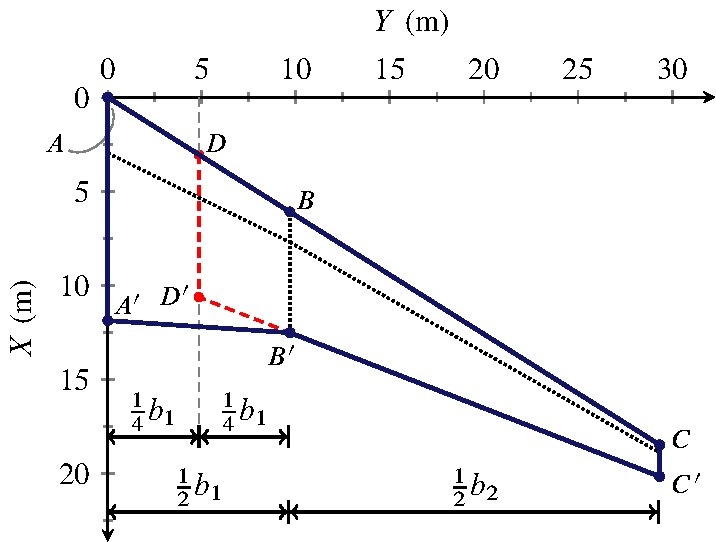
\includegraphics[width=0.72\textwidth]{Chapter_2/aerodynamic_center_of_a_cranked_wing/wing_ac_cranked_1_drawing_panels.pdf}%
  \caption{\finalhyphendemerits=1000
          \emph{Cranked} wing proposed in the example~\ref{example:Wing:Aerodynamic:Center:Cranked}.
          The inner panel $ABB'A'$, the outer panel $BCC'B'$ and the extended outer panel $DCC'D'$ are highlight
          (\emph{constructed panel}) used for the calculation of the aerodynamic center of the wing.
  }
  \label{fig:Wing:Aerodynamic:Center:Cranked:Panels}%
\end{figure}%
%-----------------------------------------------------------------------------------------------

\bigskip
From the data it is easy to obtain the law of the chords:
\[
c(Y)=
\begin{cases}
%\left\{
%\begin{array}{cl}
c_1(Y) = A_{c,1} \, Y + B_{c,1} & \text{for }\makebox[3em][r]{$0$}     \le Y \le \frac{1}{2}b_1
\\[4pt]
c_2(Y) = A_{c,2} \, \bigg(Y-\dfrac{b_1}{2}\bigg) + B_{c,2} & \text{for }\makebox[3em][r]{$\frac{1}{2}b_1$}< Y \le \frac{1}{2}b
\end{cases}
%\right.
\]
with
\[
A_{c,1}
  = \frac{c_{\mathrm{t},1} - c_{\mathrm{r},1}}{b_1/2}
  = 
    2 \frac{
      \SI[round-precision=2]{\myChordTipWingIMT}{\metre} - \SI[round-precision=2]{\myChordRootWingIMT}{\metre}
    }{
      \SI[round-precision=2]{\mySpanWingIMT}{\metre}
    }
  = \mathunderline{mydarkblue}{ \SI[round-precision=3]{\myCoeffAChordWingI}{} }
\]
\[
B_{c,1}
  = c_{\mathrm{r},1}
  = \mathunderline{mydarkblue}{ \SI[round-precision=2]{\myCoeffBChordWingIMT}{\metre} }
\]
\[
A_{c,2}
  = \frac{c_{\mathrm{t},2} - c_{\mathrm{r},2}}{b_2/2}
  = 
    2 \frac{
      \SI[round-precision=2]{\myChordTipWingIIMT}{\metre} - \SI[round-precision=2]{\myChordRootWingIIMT}{\metre}
    }{
      \SI[round-precision=2]{\mySpanWingIIMT}{\metre}
    }
  = \mathunderline{mydarkblue}{ \SI[round-precision=3]{\myCoeffAChordWingII}{} }
\]
\[
B_{c,2}
  = c_{\mathrm{r},2}
  = \mathunderline{mydarkblue}{ \SI[round-precision=2]{\myCoeffBChordWingIIMT}{\metre} }
\]
Therefore, we get
\[
c(Y)=
\begin{cases}
%\left\{
%\begin{array}{cl}
c_1(Y) = 
  \SI[round-precision=3]{\myCoeffAChordWingI}{} \, Y 
    + \SI[round-precision=2]{\myCoeffBChordWingIIMT}{\metre} 
  & \text{for}
    \makebox[3.5em][r]{$\SI[round-precision=0]{0}{\metre}$} 
      \le Y \le 
      \calcSI[round-precision=2,fixed-exponent=0,scientific-notation=fixed]{0.5*\mySpanWingIMT}{\metre}
\\[4pt]
c_2(Y) 
  = \SI[round-precision=3]{\myCoeffAChordWingII}{} \, 
    \big(
      Y
      - \calcSI[round-precision=2,fixed-exponent=0,scientific-notation=fixed]{0.5*\mySpanWingIMT}{\metre}
    \big)
    + \SI[round-precision=2]{\myCoeffBChordWingIIMT}{\metre} 
  & \text{for }
    \makebox[3.5em][r]{%
      $\calcSI[round-precision=2,fixed-exponent=0,scientific-notation=fixed]{0.5*\mySpanWingIMT}{\metre}$
    }% end-of-makebox
      < Y 
      \le \calcSI[round-precision=2,fixed-exponent=0,scientific-notation=fixed]{0.5*\mySpanWingMT}{\metre}
\end{cases}
%\right.
\]

From the figure~\ref{fig:Wing:Aerodynamic:Center:Cranked:Panels} are observed
the points $A$, $B$, $B'$ and $A'$ which define the inner portion of the wing.
The inner panel has a taper ratio
\[
\lambda_1
  =\frac{c_{\mathrm{t},1}}{c_{\mathrm{r},1}}
  =\frac{\SI[round-precision=2]{\myChordTipWingIMT}{\metre}}{\SI[round-precision=2]{\myChordRootWingIMT}{\metre}}
  =\mathunderline{mydarkblue}{ \SI[round-precision=2]{\myTaperRatioWingI}{} }
\]
a wing surface
\[
S_1 = \frac{b_1}{2} \, c_{\mathrm{r},1} \, \big( 1 + \lambda_1 \big)
  =
    \num{0.5} \cdot \SI[round-precision=1]{\mySpanWingIMT}{\metre}
      \cdot \SI[round-precision=2]{\myChordRootWingIMT}{\metre}
      \cdot \big( 1 + \SI[round-precision=2]{\myTaperRatioWingI}{} \big) 
    = \mathunderline{mydarkblue}{ \SI[round-precision=1]{\myAreaWingIMTsquared}{\metre^2} }
\]
an aspect ratio
\[
\AR_1 
  = \frac{b_1^2}{S_1}
  = \frac{\big(\SI[round-precision=1]{\mySpanWingIMT}{\metre}\big)^2}{\SI[round-precision=1]{\myAreaWingIMTsquared}{\metre^2}}
  = \mathunderline{mydarkblue}{ \num[round-precision=2]{\myAspectRatioWingI} }
\]
From these values a mean aerodynamic chord is obtained
\[
\begin{split}
\bar{c}_1 & {}= \frac{2}{3} \, c_{\mathrm{r},1} \, \frac{1+\lambda_1 + \lambda_1^2}{1+\lambda_1} \\
  & {}=
    \num{0.667} \cdot \SI[round-precision=2]{\myChordRootWingIMT}{\metre}
      \cdot 
        \frac{
          1 + \SI[round-precision=2]{\myTaperRatioWingI}{} + \SI[round-precision=2]{\myTaperRatioWingI}{}^2
        }{
          1 + \SI[round-precision=2]{\myTaperRatioWingI}{}
        }
    = \mathunderline{mydarkblue}{ \SI[round-precision=2]{\myMACWingIMT}{\metre} }
\end{split}
\]
The wing section of the inner panel having a chord $\bar{c}_1$ has a leading edge
abscissa
\[
\begin{split}
X_{\mathrm{le},\bar{c}_1} 
  & {}=
    \frac{b_1}{6} \, \frac{1+2\lambda_1}{1+\lambda_1} \tan\Lambda_\mathrm{le,1} \\[3pt]
  & {}=
    \frac{\SI[round-precision=1]{\mySpanWingIMT}{\metre}}{6}
      \cdot 
      \frac{
        1 + 2\cdot\SI[round-precision=2]{\myTaperRatioWingI}{}
      }{
        1 + \SI[round-precision=2]{\myTaperRatioWingI}{}
      }
      \cdot \tan \big( \SI[round-precision=3]{\mySweepLEWingIRAD}{\radian} \big)
    = \mathunderline{mydarkblue}{ \SI[round-precision=2]{\myXMACLEToApexWingIMT}{\metre} }
\end{split}
\]
corresponding to the station
\[
\begin{split}
Y_{\bar{c}_1} 
  & {}=
    \frac{b_1}{6} \, \frac{1+2\lambda_1}{1+\lambda_1} \\[3pt]
  & {}=
    \frac{\SI[round-precision=1]{\mySpanWingIMT}{\metre}}{6}
      \cdot 
      \frac{
        1 + 2\cdot\SI[round-precision=2]{\myTaperRatioWingI}{}
      }{
        1 + \SI[round-precision=2]{\myTaperRatioWingI}{}
      }
    = \mathunderline{mydarkblue}{ \SI[round-precision=2]{\myYMACWingIMT}{\metre} }
\end{split}
\]
along the wingspan.

Similarly, from the figure~\ref{fig:Wing:Aerodynamic:Center:Cranked:Panels} are observed
the points $B$, $C$, $C'$ and $B'$ which define the outer portion of the wing.
For the outer panel there is a taper ratio
\[
\lambda_2
  =\frac{c_{\mathrm{t},2}}{c_{\mathrm{r},2}}
  =\frac{\SI[round-precision=2]{\myChordTipWingIIMT}{\metre}}{\SI[round-precision=2]{\myChordRootWingIIMT}{\metre}}
  =\mathunderline{mydarkblue}{ \SI[round-precision=2]{\myTaperRatioWingII}{} }
\]
a wing surface
\[
S_2 = \frac{b_2}{2} \, c_{\mathrm{r},2} \, \big( 1 + \lambda_2 \big)
  =
    \num{0.5} \cdot \SI[round-precision=1]{\mySpanWingIIMT}{\metre}
      \cdot \SI[round-precision=2]{\myChordRootWingIIMT}{\metre}
      \cdot \big( 1 + \SI[round-precision=2]{\myTaperRatioWingII}{} \big) 
    = \mathunderline{mydarkblue}{ \SI[round-precision=1]{\myAreaWingIIMTsquared}{\metre^2} }
\]
and an aspect ratio
\[
\AR_2 
  = \frac{b_2^2}{S_2}
  = \frac{\big(\SI[round-precision=1]{\mySpanWingIIMT}{\metre}\big)^2}{\SI[round-precision=1]{\myAreaWingIIMTsquared}{\metre^2}}
  = \mathunderline{mydarkblue}{ \num[round-precision=2]{\myAspectRatioWingII} }
\]

Consequently, we have a mean aerodynamic  chord
\[
\begin{split}
\bar{c}_2 & {}= \frac{2}{3} \, c_{\mathrm{r},2} \, \frac{1+\lambda_2 + \lambda_2^2}{1+\lambda_2} \\
  & {}=
    \num{0.667} \cdot \SI[round-precision=2]{\myChordRootWingIIMT}{\metre}
      \cdot 
        \frac{
          1 + \SI[round-precision=2]{\myTaperRatioWingII}{} + \SI[round-precision=2]{\myTaperRatioWingII}{}^2
        }{
          1 + \SI[round-precision=2]{\myTaperRatioWingII}{}
        }
    = \mathunderline{mydarkblue}{ \SI[round-precision=2]{\myMACWingIIMT}{\metre} }
\end{split}
\]
The leading edge of the chord profile $\bar{c}_2$ is far
\[
\begin{split}
X_{\mathrm{le},\bar{c}_2} - X_B
  & {}=
    \frac{b_2}{6} \, \frac{1+2\lambda_2}{1+\lambda_2} \tan\Lambda_\mathrm{le,2} \\[3pt]
  & {}=
    \frac{\SI[round-precision=1]{\mySpanWingIIMT}{\metre}}{6}
      \cdot 
      \frac{
        1 + 2\cdot\SI[round-precision=2]{\myTaperRatioWingII}{}
      }{
        1 + \SI[round-precision=2]{\myTaperRatioWingII}{}
      }
      \cdot \tan \big( \SI[round-precision=3]{\mySweepLEWingIIRAD}{\radian} \big)
    = \mathunderline{mydarkblue}{ \SI[round-precision=2]{\myXMACLEToApexWingIIMT}{\metre} }
\end{split}
\]
longitudinally from the pointo $B$. Therefore
\[
\begin{split}
X_{\mathrm{le},\bar{c}_2} & {}= X_B + \SI[round-precision=2]{\myXMACLEToApexWingIIMT}{\metre}
  = \frac{b_1}{2} \tan \Lambda_{\mathrm{le},1} + \SI[round-precision=2]{\myXMACLEToApexWingIIMT}{\metre}
\\
  & {}= \calcSI[round-precision=2,fixed-exponent=0,scientific-notation=fixed]{
          0.5 * \mySpanWingIMT
        }{\metre}
       \cdot \tan( \SI[round-precision=3]{\mySweepLEWingIRAD}{\radian} )
      + \SI[round-precision=2]{\myXMACLEToApexWingIIMT}{\metre}
    = \calcSI[round-precision=2,fixed-exponent=0,scientific-notation=fixed]{
          0.5 * \mySpanWingIMT * tan( \mySweepLEWingIRAD )
        }{\metre}
      + \SI[round-precision=2]{\myXMACLEToApexWingIIMT}{\metre}
    = \mathunderline{mydarkblue}{ 
      \calcSI[round-precision=2,fixed-exponent=0,scientific-notation=fixed]{
          0.5 * \mySpanWingIMT * tan( \mySweepLEWingIRAD )
          + \myXMACLEToApexWingIIMT
      }{\metre}
    }
\end{split}
\]
Consequently, the station identifies the panel profile along the wingspan
chord exterior $\bar{c}_2$ is
\[
\begin{split}
Y_{\bar{c}_2} 
  & {}=
    \frac{b_1}{2} + 
    \frac{b_2}{6} \, \frac{1+2\lambda_2}{1+\lambda_2} \\[3pt]
  & {}=
    \calcSI[round-precision=2]{0.5*\mySpanWingIMT}{\metre} +
    \frac{\SI[round-precision=1]{\mySpanWingIIMT}{\metre}}{6}
      \cdot 
      \frac{
        1 + 2\cdot\SI[round-precision=2]{\myTaperRatioWingII}{}
      }{
        1 + \SI[round-precision=2]{\myTaperRatioWingII}{}
      }
    = \mathunderline{mydarkblue}{
      \calcSI[round-precision=2]{0.5*\mySpanWingIMT}{\metre} +
      \SI[round-precision=2]{\myYMACWingIIMT}{\metre} 
    }
    = \mathunderline{mydarkblue}{
      \calcSI[round-precision=2,fixed-exponent=0,scientific-notation=fixed]{0.5*\mySpanWingIMT + \myYMACWingIIMT}{\metre}
    }
\end{split}
\]

The previous calculations allow to determine the mean aerodynamic chord $\bar{c}$ of the wing,
which total surface area is
\[
S = S_1 + S_2
  = \SI[round-precision=1]{\myAreaWingIMTsquared}{\metre^2}
    = \mathunderline{mydarkblue}{
      \SI[round-precision=1]{\myAreaWingCrankedMTsquared}{\metre^2}
    }
\]
and aspect ratio
\[
\AR = \frac{b^2}{S} 
    = \frac{
        \big( \SI[round-precision=2]{\mySpanWingMT}{\meter} \big)^2
      }{
        \SI[round-precision=1]{\myAreaWingCrankedMTsquared}{\metre^2}
      }
    = \mathunderline{mydarkblue}{
      \SI[round-precision=2]{\myAspectRatioWingCranked}{}
    }
\]
The value of $\bar{c}$ is the following:
\[
\bar{c} = \frac{S_1 \, \bar{c}_1 + S_2 \, \bar{c}_2} {S_1 + S_2}
  =
  \frac{\SI[round-precision=1]{\myAreaWingIMTsquared}{\metre^2} \cdot \SI[round-precision=2]{\myMACWingIMT}{\metre} + \SI[round-precision=1]{\myAreaWingIIMTsquared}{\metre^2} \cdot \SI[round-precision=2]{\myMACWingIIMT}{\metre}}{\SI[round-precision=1]{\myAreaWingIMTsquared}{\metre^2} + \SI[round-precision=1]{\myAreaWingIIMTsquared}{\metre^2}}
    = \mathunderline{mydarkblue}{ \SI[round-precision=2]{\myMACWingCrankedMT}{\metre} }
\]
Being in this case
$\bar{c} < c_{\mathrm{t},1}=\SI[round-precision=2]{\myMACWingIMT}{\metre}$,
the station is determined
\[
  Y_{\bar{c}} 
    = \frac{\bar{c} - B_{c,1}}{A_{c,1}}
    = \frac{
        \SI[round-precision=2]{\myMACWingCrankedMT}{\metre} 
        - \SI[round-precision=2]{\myCoeffBChordWingIMT}{\metre}
      }{
        \SI[round-precision=3]{\myCoeffAChordWingI}{}
      }
    = \mathunderline{mydarkblue}{
      \SI[round-precision=2]{\myYYMACWingCrankedMT}{\metre}
    }
\]
along the wingspan corresponding to the chord profile $\bar{c}$. This profile
has leading edge of abscissa
\[
X_{\mathrm{le},\bar{c}} 
  % = \frac{\bar{c} - B_{c,1}}{A_{c,1}} \tan \Lambda_{\mathrm{le},1}
  = Y_{\bar{c}} \tan \Lambda_{\mathrm{le},1}
  =
%	\frac{
%	\SI[round-precision=2]{\myMACWingCrankedMT}{\metre}
%	-
%	\SI[round-precision=2]{\myCoeffBChordWingIMT}{\metre}
%	}{
%	\SI[round-precision=2]{\myCoeffAChordWingI}{}
%	}
   \SI[round-precision=2]{\myYYMACWingCrankedMT}{\metre}
   \cdot
	\tan \big( \SI[round-precision=3]{\mySweepLEWingIRAD}{\radian} \big)
	= \mathunderline{mydarkblue}{ \SI[round-precision=2]{\myXXMACLEToApexWingCrankedMT}{\metre} }
\]
% 
In the figure~\ref{fig:Wing:Aerodynamic:Center:Cranked:MAC}
the drawing of the assigned planform is shown where the chords are indicated $\bar{c}_1$, $\bar{c}_2$ e $\bar{c}$
and the distances $X_{\mathrm{le},\bar{c}}$ and $Y_{\bar{c}}$.

\medskip
At this point the aerodynamic center of the assigned wing is calculated.
The graphical method used in the example~\ref{example:Wing:Aerodynamic:Center:Of:A:Finite:Wing}
for determining the aerodynamic center of a straight-edged wing
can be applied here to each of the two wing panels.
Unlike the case of a simple wing, for a wing \emph{cranked} we have to derive
an external panel  \emph{extended} --- said \emph{constructed outer panel} --- as shown in
figures~\ref{fig:Wing:Aerodynamic:Center:Cranked:Panels}
and~\ref{fig:Wing:Aerodynamic:Center:Cranked:Panels:AC}. 
It is given by extending the leading and trailing edges
of panel~2 towards the inside,
starting, respectively, from the points $B$ and $B'$, until we get to the points $D$ and $D'$ the parallel line
to the axis $X$ of equation $Y=\frac{1}{4}b_1$.
Therefore, the inner panel is considered in the following calculations
$\mathcal{P}_1=ABB'A'$ annd,
instead of the panel $\mathcal{P}_2=BCC'B$,
the extended outer panel $\mathcal{P}_{2'}=DCC'D'$.

As for the inner panel $\mathcal{P}_{1}$,
from the data and the figure
~\ref{fig:Wing:Ac:K:One:Plots}
we can see
\[
\lambda_1=\SI[round-precision=2]{\myTaperRatioWingI}{}
%
%\quad \Longrightarrow \quad
%\quad \begin{array}{@{}c@{}} \myIconGraph \\[-4pt] \Longrightarrow \end{array} \quad
\adjustbox{center=4em}{%
  \adjustbox{lap=\width}{\raisebox{2.2ex}[0pt][0pt]{\myIconGraph}}$\Longrightarrow$%
}
%
K_{1,\mathcal{P}_{1}}
  = \mathunderline{mydarkblue}{ \SI[round-precision=3]{\myKOneACDatcomWingI}{} }
\]
from the figure~\ref{fig:Wing:Ac:K:Two:Plots}
we can see
\[
\Lambda_\mathrm{le,1} = \SI[round-precision=1]{\mySweepLEWingIDEG}{\deg}\;,\;\,
\AR_1 = \SI[round-precision=1]{\myAspectRatioWingI}{}\;,\;\,
\lambda_1=\SI[round-precision=2]{\myTaperRatioWingI}{}
%\quad \Longrightarrow \quad
%\quad \begin{array}{@{}c@{}} \myIconGraph \\[-4pt] \Longrightarrow \end{array} \quad
\adjustbox{center=4em}{%
  \adjustbox{lap=\width}{\raisebox{2.2ex}[0pt][0pt]{\myIconGraph}}$\Longrightarrow$%
}
%
K_{2,\mathcal{P}_{1}} 
  = \mathunderline{mydarkblue}{ \SI[round-precision=3]{\myKTwoACDatcomWingI}{} }
\]
from the figure~\ref{fig:Wing:Ac:X:AC:From:Apex:Plots}
we obtain
\[
\Lambda_\mathrm{le,1} = \SI[round-precision=1]{\mySweepLEWingIDEG}{\deg}\;,\;\,
\Mach = \SI[round-precision=2]{\myMach}{}\;,\;\,
\AR_1 = \SI[round-precision=1]{\myAspectRatioWingI}{}\;,\;\,
\lambda_1=\SI[round-precision=2]{\myTaperRatioWingI}{}
%
%\quad \Longrightarrow \quad
%\quad \begin{array}{@{}c@{}} \myIconGraph \\[-4pt] \Longrightarrow \end{array} \quad
\adjustbox{center=4em}{%
  \adjustbox{lap=\width}{\raisebox{2.2ex}[0pt][0pt]{\myIconGraph}}$\Longrightarrow$%
}
%
\left.
\frac{X'_{\mathrm{ac}}}{c_\mathrm{r}}\right|_{\mathcal{P}_{1}}
  = \mathunderline{mydarkblue}{ \SI[round-precision=3]{\myXACOverChordRootDatcomWingI}{} }
\]
%
It is thus obtained
\[
\left.
\frac{x_{\mathrm{ac}}}{\bar{c}}\right|_{\mathcal{P}_{1}} 
  = K_{1,\mathcal{P}_{1}} 
    \left( 
      \left.\frac{X'_{\mathrm{ac}}}{c_\mathrm{r}}\right|_{\mathcal{P}_{1}} 
        - K_{2,\mathcal{P}_{1}}
    \right)
  = \SI[round-precision=3]{\myKOneACDatcomWingI}{} \,
    \Big(  
      \SI[round-precision=3]{\myXACOverChordRootDatcomWingI}{} 
        - \SI[round-precision=3]{\myKTwoACDatcomWingI}{}  
    \Big)
  = \mathunderline{mydarkblue}{ \SI[round-precision=3]{\myXsiACWingI}{} } 
\]

%-----------------------------------------------------------------------------------------------
\begin{figure}
  [t]%[H]%[!htbp]
  %\centering
  %\checkoddpage
  %\centering
    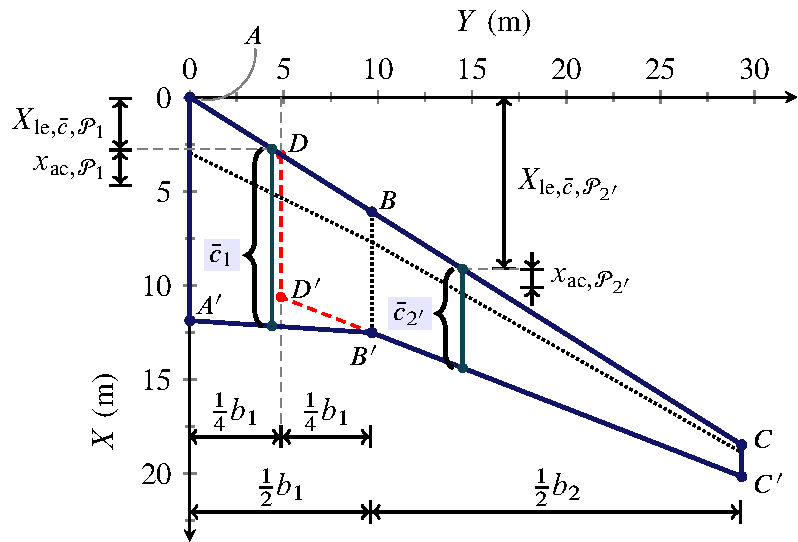
\includegraphics[width=0.78\textwidth]{Chapter_2/aerodynamic_center_of_a_cranked_wing/wing_ac_cranked_1_drawing_panels_ac}
  \caption{\finalhyphendemerits=1000
          Aerodynamic centers of the panels
          $\mathcal{P}_1=ABB'A'$ and $\mathcal{P}_{2'}=DCC'D'$.
  }
  \label{fig:Wing:Aerodynamic:Center:Cranked:Panels:AC}%
\end{figure}

%-----------------------------------------------------------------------------------------------

As for the inner panel $\mathcal{P}_{2'}$,
we get
\[
b_{2'} = 2 \left( \frac{1}{2}b_2 + \frac{1}{4}b_1 \right)
  =
    2 \big(
    \calcSI[round-precision=2,fixed-exponent=0,scientific-notation=fixed]{0.5*\mySpanWingIIMT}{\metre}
    +
    \calcSI[round-precision=2,fixed-exponent=0,scientific-notation=fixed]{0.25*\mySpanWingIMT}{\metre}
    \big)
  = \SI[round-precision=2]{\mySpanWingIIPrimeMT}{m}
\]
\[
c_{\mathrm{r},2'}
  = A_{c,2} \, \bigg( - \frac{1}{4}b_1 \bigg) + B_{c,2}
  =
    \SI[round-precision=3]{\myCoeffAChordWingII}{} \, 
    \big(
      - \calcSI[round-precision=2,fixed-exponent=0,scientific-notation=fixed]{0.25*\mySpanWingIMT}{\metre}
    \big)
    + \SI[round-precision=2]{\myCoeffBChordWingIIMT}{\metre}
  = \SI[round-precision=2]{\myChordRootWingIIPrimeMT}{m}
\]
\[
\lambda_{2'}
  =\frac{c_{\mathrm{t},2}}{c_{\mathrm{r},2'}}
  =\frac{\SI[round-precision=2]{\myChordTipWingIIMT}{\metre}}{\SI[round-precision=2]{\myChordRootWingIIPrimeMT}{\metre}}
  =\mathunderline{mydarkblue}{ \SI[round-precision=2]{\myTaperRatioWingIIPrime}{} }
\]
\[
S_{2'} 
  = \frac{b_{2'}}{2} \, c_{\mathrm{r},{2'}} \, \big( 1 + \lambda_{2'} \big)
  =
    \num{0.5} \cdot \SI[round-precision=1]{\mySpanWingIIPrimeMT}{\metre}
      \cdot \SI[round-precision=2]{\myChordRootWingIIPrimeMT}{\metre}
      \cdot \big( 1 + \SI[round-precision=2]{\myTaperRatioWingIIPrime}{} \big) 
    = \mathunderline{mydarkblue}{ \SI[round-precision=1]{\myAreaWingIIPrimeMTsquared}{\metre^2} }
\]
\[
\AR_{2'} 
  = \frac{b_{2'}^2}{S_{2'}}
  = \frac{\big(\SI[round-precision=1]{\mySpanWingIIPrimeMT}{\metre}\big)^2}{\SI[round-precision=1]{\myAreaWingIIPrimeMTsquared}{\metre^2}}
  = \mathunderline{mydarkblue}{ \num[round-precision=2]{\myAspectRatioWingIIPrime} }
\]


From the data and the figure~\ref{fig:Wing:Ac:K:One:Plots}
we can see
\[
\lambda_{2'}=\SI[round-precision=2]{\myTaperRatioWingIIPrime}{}
%
%\quad \Longrightarrow \quad
%\quad \begin{array}{@{}c@{}} \myIconGraph \\[-4pt] \Longrightarrow \end{array} \quad
\adjustbox{center=4em}{%
  \adjustbox{lap=\width}{\raisebox{2.2ex}[0pt][0pt]{\myIconGraph}}$\Longrightarrow$%
}
%
K_{1,\mathcal{P}_{2'}}
  = \mathunderline{mydarkblue}{ \SI[round-precision=3]{\myKOneACDatcomWingII}{} }
\]
from figure~\ref{fig:Wing:Ac:K:Two:Plots}
we can obtain
\[
\Lambda_\mathrm{le,2} = \SI[round-precision=1]{\mySweepLEWingIIDEG}{\deg}\;,\;\,
\AR_{2'} = \SI[round-precision=1]{\myAspectRatioWingIIPrime}{}\;,\;\,
\lambda_{2'}=\SI[round-precision=2]{\myTaperRatioWingIIPrime}{}
%\quad \Longrightarrow \quad
%\quad \begin{array}{@{}c@{}} \myIconGraph \\[-4pt] \Longrightarrow \end{array} \quad
\adjustbox{center=4em}{%
  \adjustbox{lap=\width}{\raisebox{2.2ex}[0pt][0pt]{\myIconGraph}}$\Longrightarrow$%
}
%
K_{2,\mathcal{P}_{2'}} 
  = \mathunderline{mydarkblue}{ \SI[round-precision=3]{\myKTwoACDatcomWingII}{} }
\]
from figure~\ref{fig:Wing:Ac:X:AC:From:Apex:Plots}
we can see
\[
\Lambda_\mathrm{le,2} = \SI[round-precision=1]{\mySweepLEWingIIDEG}{\deg}\;,\;\,
\Mach = \SI[round-precision=2]{\myMach}{}\;,\;\,
\AR_{2'} = \SI[round-precision=1]{\myAspectRatioWingIIPrime}{}\;,\;\,
\lambda_{2'}=\SI[round-precision=2]{\myTaperRatioWingIIPrime}{}
%
%\quad \Longrightarrow \quad
%\quad \begin{array}{@{}c@{}} \myIconGraph \\[-4pt] \Longrightarrow \end{array} \quad
\adjustbox{center=4em}{%
  \adjustbox{lap=\width}{\raisebox{2.2ex}[0pt][0pt]{\myIconGraph}}$\Longrightarrow$%
}
%
\left.
\frac{X'_{\mathrm{ac}}}{c_\mathrm{r}}\right|_{\mathcal{P}_{2'}}
  = \mathunderline{mydarkblue}{ \SI[round-precision=3]{\myXACOverChordRootDatcomWingII}{} }
\]

At this point we can calculate the quantity
\[
\frac{X_{\mathrm{ac}}}{c_\mathrm{r}}
  = \frac{
    \left.\dfrac{X'_{\mathrm{ac}}}{c_\mathrm{r}}\right|_{\mathcal{P}_{1}}
      \, S_{1} \, C_{L_\mathlarger{\alpha}}\Big|_{\mathcal{P}_{1}}
    +
    \left.\dfrac{X'_{\mathrm{ac}}}{c_\mathrm{r}}\right|_{\mathcal{P}_{2'}}
      \, S_{2'} \, C_{L_\mathlarger{\alpha}}\Big|_{\mathcal{P}_{2'}}
  }{
    S_{1} \, C_{L_\mathlarger{\alpha}}\Big|_{\mathcal{P}_{1}} 
    + S_{2'} \, C_{L_\mathlarger{\alpha}}\Big|_{\mathcal{P}_{2'}} 
  }
\]
after determining the gradient of the lift coefficient for each panel.
For the geometric characteristics of the panels $\mathcal{P}_{1}$ and
$\mathcal{P}_{2'}$ the two gradients can be estimated as follows:
\[
C_{L_\mathlarger{\alpha}}\Big|_{\mathcal{P}_{1}}
  =
  \frac{
    a_0 \cos \Lambda_{\mathrm{le,1}}
  }{
    \sqrt{
      1 - \Mach^2 \cos^2 \Lambda_{\mathrm{le,1}}
        + \left( \dfrac{ a_0 \cos \Lambda_{\mathrm{le,1}} }{ \pi \AR_1} \right)^2
    }
    +
    \dfrac{ a_0 \cos \Lambda_{\mathrm{le,1}} }{ \pi \AR_1}
  }
\]
\[
C_{L_\mathlarger{\alpha}}\Big|_{\mathcal{P}_{2'}}
  =
  \frac{
    a_0 \cos \Lambda_{\mathrm{le,2}}
  }{
    \sqrt{
      1 - \Mach^2 \cos^2 \Lambda_{\mathrm{le,2}}
        + \left( \dfrac{ a_0 \cos \Lambda_{\mathrm{le,2}} }{ \pi \AR_{2'}} \right)^2
    }
    +
    \dfrac{ a_0 \cos \Lambda_{\mathrm{le,2}} }{ \pi \AR_{2'}}
  }
\]
with
\[
a_0 = 
  \frac{
    \SI[round-precision=3]{\myCLAlphaAtMACWingRAD}{\radian^{-1}}
  }{
    \sqrt{ 1 - \Mach^2 \cos^2 \Lambda_{\mathrm{le,1}} }
  }
  \qquad (\, \Lambda_{\mathrm{le,1}} = \Lambda_{\mathrm{le,2}} \,)
\]
From the data of the problem it is easy to verify that we have
\[
C_{L_\mathlarger{\alpha}}\Big|_{\mathcal{P}_{1}}
  = \SI[round-precision=3]{\myCLAlphaPolhamusWingIRAD}{\radian^{-1}}
  = \SI[round-precision=4]{\myCLAlphaPolhamusWingIDEG}{\deg^{-1}}
\,,
\qquad
C_{L_\mathlarger{\alpha}}\Big|_{\mathcal{P}_{2'}}
  = \SI[round-precision=3]{\myCLAlphaPolhamusWingIIRAD}{\radian^{-1}}
  = \SI[round-precision=4]{\myCLAlphaPolhamusWingIIDEG}{\deg^{-1}}
\]
Therefore, it is obtained
\[
\frac{X_{\mathrm{ac}}}{c_\mathrm{r}}
  = \frac{
    \SI[round-precision=3]{\myXACOverChordRootDatcomWingI}{}
    \cdot \SI[round-precision=3]{\myCLAlphaPolhamusWingIRAD}{\radian^{-1}}
    \cdot \SI[round-precision=1]{\myAreaWingIMTsquared}{\metre^{2}}
    +
    \SI[round-precision=3]{\myXACOverChordRootDatcomWingII}{}
    \cdot \SI[round-precision=3]{\myCLAlphaPolhamusWingIIRAD}{\radian^{-1}}
    \cdot \SI[round-precision=1]{\myAreaWingIIPrimeMTsquared}{\metre^{2}}
  }{
    \SI[round-precision=3]{\myCLAlphaPolhamusWingIRAD}{\radian^{-1}}
    \cdot \SI[round-precision=1]{\myAreaWingIMTsquared}{\metre^{2}}
    +
    \cdot \SI[round-precision=3]{\myCLAlphaPolhamusWingIIRAD}{\radian^{-1}}
    \cdot \SI[round-precision=1]{\myAreaWingIIPrimeMTsquared}{\metre^{2}}  
  }
  = 
  \mathunderline{mydarkblue}{ \SI[round-precision=3]{\myXACOverChordRootDatcomWing}{} }
\]

For a \emph{cranked} wing this is the decisive result, which allows
obtain
\[
X_{\mathrm{ac}} = \frac{X_{\mathrm{ac}}}{c_\mathrm{r}} \, c_{\mathrm{r},1}
  = \SI[round-precision=3]{\myXACOverChordRootDatcomWing}{}
    \cdot \SI[round-precision=2]{\myChordRootWingIMT}{\metre}
  = \SI[round-precision=2]{\myACWingToApexWingMT}{\metre} 
\]
i.e.
\[
\frac{x_{\mathrm{ac}}}{\bar{c}}
  = 
  \frac{
    X_{\mathrm{ac}} - X_{\mathrm{le},\bar{c}}
  }{
    \bar{c}
  }
  =
  \frac{
    \SI[round-precision=2]{\myACWingToApexWingMT}{\metre}
      - \SI[round-precision=2]{\myXXMACLEToApexWingCrankedMT}{\metre}
  }{
    \SI[round-precision=2]{\myMACWingCrankedMT}{\metre}
  }
  =
  \mathunderline{mydarkblue}{ \SI[round-precision=3]{\myXsiACWing}{} }  
\]

The aerodynamic center of coordinates $(X_\mathrm{ac},0)$
is represented in the figure~\ref{fig:Wing:Aerodynamic:Center:Cranked:Results}.

%-----------------------------------------------------------------------------------------------
\begin{figure}[t]%[H]%[!htbp]
  %\centering
  %\checkoddpage
  %\centering
    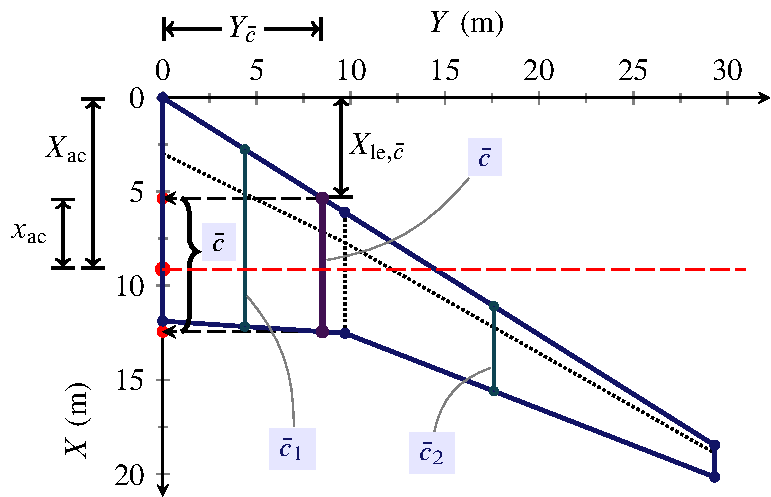
\includegraphics[width=0.78\textwidth]{Chapter_2/aerodynamic_center_of_a_cranked_wing/wing_ac_cranked_1_drawing.pdf}
  \caption{\finalhyphendemerits=1000
         Aerodynamic center of the wing proposed in the example~\ref{example:Wing:Aerodynamic:Center:Cranked}. The dashed axis,
           parallel to the axis $Y$and passing through the wing aerodynamic center
           is the pitch axis around which the moment coefficient
           of the wing is constant as the angle of attack of the flow varies:
          \smash{$\partial C_{\mathcal{M}_\mathlarger{\mathrm{ac}}}/\partial\alpha = 0$}.
  }
  \label{fig:Wing:Aerodynamic:Center:Cranked:Results}%
\end{figure}
\end{myExampleX}
\end{document}